\chapter{Mathematical preliminaries}
    
   \section{Abstract vector spaces}
   In previous courses, the notion of a \textbf{vector} was introduced as being an n-tuple of ordered numbers ( either real or complex). However, one can have a more general definition for a vector as being an element of a \textbf{vector space}. A vector space is a set that  satisfies the following property\\
   Let $ \mathcal{V}$ be a vector space, and $\lvert \psi \rangle$ and $\lvert \phi \rangle$ are elements of it . Then :
   \begin{equation}
   	 \alpha  \lvert \psi \rangle +  \beta \lvert \phi \rangle, 
   	 \label{linear}
   \end{equation}
   is also an element of that vector space, where $ \alpha$ and $ \beta$ are complex or real numbers. 
   The expression \eqref{linear} is called the \textbf{superposition} of the vectors $\lvert \psi \rangle$ and $\lvert \phi \rangle$. \\ The dimension of $ \mathcal{V}$ could either be finite , countably infinite or uncountably infinite ( see next section). For  finite dimensional- or countably infinite- vector spaces. It is possible to represent a vector $\lvert \psi \rangle$ as a column matrix :
   \begin{equation}
   \lvert f \rangle \Leftrightarrow \left( \begin{array}{c}
f_1\\ f_2\\ f_3\\\vdots
   \end{array}\right) 
   \end{equation}
   We can represent the components of the above vector in what-so-called a \textbf{spike diagram } representing the magnitude of each component of the vector $ \lvert \psi \rangle $. 
   \begin{figure}[h!]
   	\centering
   	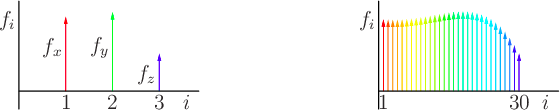
\includegraphics[width=0.9 \textwidth]{./figures/spike}
   	\caption{ Spike digram of a vector in 3 dimensional vector space, and 30 dimensional one. }
   \end{figure}
   	\section{Functions as vectors}
   	It may seem unfamiliar to most readers that functions could be considered as vectors of an uncountably infinite dimensional vector space. In order to see this, we use the spike diagrams discussed above.This time using a continuous parameter $x$  taking real-number values instead of the discrete index $i$. The spike digram for such vector would look like:
   	   \begin{figure}[h!]
   	   	\centering
   	   	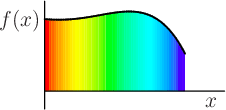
\includegraphics[width=0.5 \textwidth]{./figures/inf}
   	   	\caption{ Spike digram of a vector having infinite components}
   	   \end{figure}
 In fact, this spike digram looks familiar to the classical graph of a real-valued function $ f(x)$:
 \begin{figure}[h!]
 	\centering
 	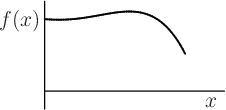
\includegraphics[width=0.5 \textwidth]{./figures/func}
 	\caption{ Classical graph of a function $ f(x)$}
 \end{figure}
 in this way, a function is just a single vector in an infinite dimensional space. It should be noted that to make the transition to infinite dimensions mathematically meaningful, you need to impose some smoothness constraints on the function. Typically, it is required that the function is continuous, or at least integrable in some sense. These details are not important for our purpose, thus we shall not discuss them further.
\section{Dual spaces and inner product}
One may define a map $\langle f\arrowvert$ that sends a vector $\lvert \phi \rangle$ in $ \mathcal{V}$ to the real or complex numbers. Defined as - for finite dimensional vector spaces or countably infinite ones:
\begin{equation}
\langle f\arrowvert \phi \rangle = \sum_i f_i \phi_i 
\end{equation}
or for functions \footnote{ The star resembles the complex conjugation $f(x)^*$}:
\begin{equation}
\langle f\arrowvert \phi \rangle = \int dx f(x)^* \phi(x)
\end{equation}
We can easily show that the set of such maps \marginpar{ sometimes they are called linear functionals} form a vector space themselves, which we call the \textbf{dual} vector space and denoted by $ \mathcal{V}^*$. Moreover, the operation between a vector and a (dual) vector is called \textbf{inner product }. \\
\subsection{The Bra-Ket notation}
Every vector space has its dual. In the notation adopted in quantum mechanics, and invented by Paul Dirac. A member of a vector space is called a \textbf{Ket} and denoted by $ \arrowvert \psi \rangle$, as we have seen, for discrete components it is represented as a column matrix .On the other hand, the elements of the dual space are denoted by a \textbf{Bra} $\langle f \arrowvert$ in Dirac notation. And represented as a row matrix: \footnote{ The inner product is carried like matrix multiplication between a row and a column}
   \begin{equation}
 \langle f  \lvert \Leftrightarrow \left( \begin{array}{cccc}
   f_1^*& f_2^*& f_3^*&\cdots
   \end{array}\right) 
   \end{equation}
   The notation adopted is known as the \textbf{Bra-Ket notation }. Since for every vector space there is a dual space. One may turn a Ket vector into a Bra vector, by a one-to-one map. Hence defining the inner product in the vector space itself, calling it an \textbf{inner-product space}.\\
	Two vectors  $\lvert \psi \rangle$ and $\lvert \phi \rangle$ are called \textbf{orthogonal} if and only if :
   	\[
   	\langle \phi| \psi \rangle = 0 
   	\]
\subsection{Normed spaces}
In a similar sense to the magnitude of a vector in the space ( like velocity), we can extend this notion to \textit{any} vector with the norm function. $ \Arrowvert \cdot \Arrowvert$ . There are many ways one can define the norm of a vector. However, we are only interested in the norm defined by the inner product:
\begin{equation}
\Arrowvert \psi  \Arrowvert \equiv\sqrt{\langle \psi | \psi \rangle}
\label{norm}
\end{equation}
Note that the norm is always a\textbf{ real number }. Vectors with a unit norm is called \textbf{normal vectors }.
\section{Hilbert space}
An inner product vector space $ \mathcal{H}$, with a norm defined in \eqref{norm}, in addition to another property called \textit{completeness} \footnote{ complete vector space is a space that all Cauchy sequences converge}is called a \textbf{Hilbert space}. Hilbert spaces are extremely important in quantum mechanics. They replace the phase spaces of classical mechanics. Hilbert spaces can be finite dimensional or  infinite dimensional ( both cases we call it \textbf{separable} Hilbert spaces), the latter infinite dimensional space might have either continuous and discrete \textit{representations}. \\
\subsection{Basis of a Hilbert space}
We can express any vector in the Hilbert space as a linear superposition of $\dim{\mathcal{H}}$ other vectors. Hence, it is possible to construct orthonormal basis for a Hilbert space. You need as many of them as the dimension of the vector space itself. 
Given a vector $ | \psi \rangle$ in the Hilbert space having a set of orthonormal basis $ S= \{ | e_i\rangle\}_i$, $ | \psi \rangle$ is uniquely expressed in terms of the basis $S$ :
\begin{equation}
| \psi \rangle = \sum_i \langle e_i| \psi \rangle \;  |e_i\rangle
\label{decomp}
\end{equation}
The coefficients $ c_j = \langle e_j| \psi \rangle$ is sometimes called \textbf{Fourier coefficients}. We can have the same argument for the Bra-vectors:
\begin{equation}
\langle\psi| = \sum_i \langle \psi| e_i \rangle \;  \langle e_i|
\end{equation}
The basis satisfy\footnote{There is a fundamental difference by what we mean by basis here and the conventional basis tough in Classical mechanics The basis we use are called Schauder basis, whilst the latter is known as Hamel basis}:
\begin{equation}
\langle e_i|e_j\rangle = \delta_{ij}
\end{equation}
For function spaces, the basis have continuous parameter  $x$ instead of a discrete index the basis therefore are denoted by $ |x\rangle$, for all $x$ a real number. A function $ \phi$ is written as :
\[
\phi(x) = \langle x| \phi \rangle
\] 
Instead of using the Bra-Ket notation for functions, we shall only denote them by $ \phi(x)$.\\
Note that we need some-sort of structure in the Hilbert space to insure that \eqref{decomp} converges if the sum is infinite. We call the Hilbert space in with the series of this type the $ \ell^2$ space, or the space of square-summable sequences. Moreover, the integrals used in this course - and in quantum mechanics in general- are known as the \textit{Lebesgue integrals }, they are different from Riemann integrals defined in calculus courses.\\
 Here, we have illustrated the most relevant properties of Hilbert spaces that concern us in the study of introductory quantum mechanics. A lot of mathematical details and rigour has been spared in this lecture. It is urged from the reader to conduct a further reading in the theory of Hilbert space; please consult: \textit{Functional Analysis} by M. Reed and B. Simon.\\
 	 
 	   \section{The space L$^2$}
 	   Functions form a vector space, as we have seen previously, nevertheless, we need to imply an additional restriction on functions in order to form a Hilbert space. Let $ \phi(x)$  be a function defined on the interval $ [a,b]$, the norm of this function is defined to be - in accordance to the formal definition of the norm- :
 	   \begin{equation}
 	   \lVert \phi(x) \rVert= \sqrt{\int_a ^b \phi(x)^* \phi(x) \,dx}
 	   \end{equation}
 	   For the norm to exist, the function $\phi(x)$ needs to be \textbf{square integrable} on the interval $ [a,b]$. It is not hard to show that the set of square-integrable functions on the same interval form a Hilbert space. This Hilbert space is known as the $ L^2( R; d\mu)$ space. It reads; the space of square-integrable function on the interval/Region $R$ \footnote{ Functions of $L^2$ could be of several variables, real or complex-valued}, with respect to the measure $ d\mu$. By measure we mean the volume element that we integrate over. In 1-D case $ d\mu =dx$.  Sometimes, one wishes to define a \textit{weight} $w(x)$ for the space, but this is out of the scope of this course.\\ 
 	   The space $L^2$  can have basis of orthogonal, and normalised functions $ ( u_1(x), u_2(x), \dots)$ depending on the interval of interest. For example the classical orthogonal polynomials including:
 	   \begin{itemize}
 	   	\item Hermite polynomials:
 	   	\begin{equation}
 	   	H_n(x) = K_n^{-1} e^{x^2} \dfrac{d^n}{dx^n}\left( e^{-x^2}\right) .
 	   	\end{equation}
 	   	They could form  basis for the space $L^2(-\infty, + \infty; dx)$. 
 	  
 	   \item Legendre polynomials:
 	   \begin{equation}
 	   L^\nu _n = K^{-1}_n x^-\nu e^x \dfrac{d^n}{dx^n}\left( x^{ \nu +1} e^x\right) .
 	   \end{equation}
 	   	They could form  basis for the space $L^2(0, + \infty; dx)$.
 	   	\item Legendre polynomials ( of the first kind):
 	   	\begin{equation}
 	   	P_n = K^{-1}_n \dfrac{d^n}{dx^n}\left( 1-x^2\right) 
 	   	\end{equation}
 	   		They could form  basis for the space $L^2(0, 1; dx)$.
 	    \end{itemize}
 	    The second example of$L^2$ spaces, are the ones used in Fourier analysis. Where $ \cos(nkx)$ and $ \sin( nkx)$ form an orthonormal basis for a given $L^2$ space with an interval $L$. Recall that we can expand any function in a Fourier series :
 	    \begin{equation}
 	    f(x) = \sum_{n =0} ^{\infty} A_n \cos(\frac{n \pi x}{L}) + B_n \sin(\frac{n \pi x}{L})
 	    \end{equation}
 	    Where :
 	    \begin{align}
 	    A_n = \int_0 ^L f(x) \cos(\frac{n \pi x}{L}) dx \\
 	    B_n = \int_0 ^L f(x) \sin(\frac{n \pi x}{L}) dx
 	    \end{align}
 	    Or expanding the function in a continuous basis ( Fourier integral).
 	   \paragraph{Note}
 	    Advanced readers might not find the discussion in this lecture formal neither accurate enough, as discussing mathematical rigour of Hilbert spaces is very distant from the course aims. 
 \section{ Outer product}
 For a finite-dimensional vector space, the outer product can be understood as simple matrix multiplication:
 \[ |\phi \rangle \, \langle \psi | {\doteq \!\,}
 \begin{pmatrix} \phi_1 \\ \phi_2 \\ \vdots \\ \phi_N \end{pmatrix}
 \begin{pmatrix} \psi_1^* & \psi_2^* & \cdots & \psi_N^* \end{pmatrix}
 = \begin{pmatrix}
 \phi_1 \psi_1^* & \phi_1 \psi_2^* & \cdots & \phi_1 \psi_N^* \\
 \phi_2 \psi_1^* & \phi_2 \psi_2^* & \cdots & \phi_2 \psi_N^* \\
 \vdots & \vdots & \ddots & \vdots \\
 \phi_N \psi_1^* & \phi_N \psi_2^* & \cdots & \phi_N \psi_N^* \end{pmatrix}
 \]
 The outer product is an N$\times$N matrix. 
 \section{Linear operators}
 The term 'linear operator' is used in many contexts, in quantum mechanics however, we are interested -mainly-  in  linear operators, acting on a Hilbert space. Linear operators are maps from a Hilbert space to itself ( known mathematically as Endomorphisms ). In simple words, they send 'kets' to 'kets'. Operators \footnote{ we shall always mean linear operator when we use the term operator from now on} are represented as square matrices ( for finite dimensional or countably infinite dimensional Hilbert spaces). Hence, all the algebra of matrices will apply to operators. Such as :
 \subsection{The algebra of operators}
 \begin{enumerate}
 	\item Linearity:\\
 	Let $\hat{A}$ and $ \hat{B}$ be operators acting on the Hilbert space $ \mathcal{H}$,$ \alpha$ and $ \beta$ are scalars, and $ | \psi \rangle $ and  $ | \phi \rangle$ be vectors in $ \mathcal{H}$. Then the following properties hold:
 	\begin{equation}
 	(\alpha \hat{A}+ \beta \hat{B}) | \psi\rangle = \alpha (\hat{A} | \psi\rangle)+ \beta ( \hat{B} |\psi\rangle)
 	\end{equation}
 	Moreover:
 	\begin{equation}
 	\hat{A}	(\alpha | \psi\rangle+ \beta  | \phi\rangle ) = \alpha (\hat{A} | \psi\rangle)+ \beta ( \hat{A} |\phi\rangle)
 	\end{equation}
 	A result from above :
 	\begin{equation}
 	\hat{A} | \psi\rangle = \sum_i \langle i|\psi \rangle\left(  \hat{A} | i \rangle\right) 
 	\end{equation}
 	\item Eigenvalue:\\
 	A scalar $ \lambda $ is called an \textbf{eigenvalue} if it satisfied the equation:
 	\begin{equation}
 	\hat{A} | \psi\rangle = \lambda  | \psi\rangle
 	\end{equation}
 	Called the\textbf{ eigenvalue equation,} and the vector $ | \psi\rangle$ is called an \textbf{eigenket}/ \textbf{eigenvector}. 
 	This equation is equivalent to :
 	\begin{equation}
 	\det\left( \hat{A} - \lambda \hat{I}\right)  =0 
 	\end{equation}
 	For $ \hat{I}$ or just $ I$ being the identity operator. 
 	An important result from this property is the spectral decomposition, that we shall discuss later in this lecture.
 	\item Self-adjointness ( Hermitian operators)\\
 	Let $ \hat{A}$ be an operator, then $ \hat{A}^\dagger$ is the \textbf{hermitian conjugate} of this operator  It is simply the hermitian matrix in the matrix representation of $ \hat{A}$ . The hermitian conjugate acts on the dual space of $ \mathcal{H}$ ( acts on the Bras).  The following properties for the hermitian conjugation are listed below ( for reminding)
 	\begin{itemize}
 		\item $\left( \hat{A}^\dagger\right) ^\dagger = \hat{A}$ – involutiveness\\
 		\item If an inverse for the operator exists then:
 		\[
 		\left( \hat{A}^{-1}\right) ^\dagger = \left( \hat{A}^{\dagger}\right) ^{-1} 
 		\]
 		\item Antilinearity:
 		\[
 		\left( \alpha \hat{A}+ \beta \hat{B}\right) ^\dagger = \alpha^* \hat{A}^\dagger + \beta^* \hat{B}^\dagger 
 		\]
 		\item $ (\hat{A}\hat{B})^\dagger = \hat{B}^\dagger \hat{A}^\dagger $.
 	\end{itemize}
 	An operator is called \textbf{self-adjoint }, if it is equal to its hermitian conjugate:
 	\[
 	\hat{A}^\dagger = \hat{A}
 	\]
 	In other words, it acts both on the Kets and on the Bras.
 	An important theorem for self-adjoint operators is stated below:\\
 	\textit{ All the  eigenvalues for a self-adjoint operator are real }
 \end{enumerate}
 Other properties of the matrices can be revised from a linear algebra book.
 \section{Spectral theorem}
 An important result from linear algebra is the spectral decomposition of an operator in terms of its eigenvalues and eigenvectors. If the set eigenvectors $\{ |u_1\rangle,|u_2\rangle, |u_3\rangle \cdots \}$ form a basis for the Hilbert space, and the set of eigenvalues $\{ \lambda_i\}$ satisfying:
 \begin{equation}
 \hat{A} | u_j \rangle = \lambda_j | u_j\rangle
 \end{equation}
 Then the operator $ \hat{A}$ is decomposed as follows:
 \begin{equation}
 \hat{A} = \sum_i  \lambda_i | u_i \rangle\langle u_i | 
 \end{equation}
 Note that the outer product $| u_i \rangle\langle u_i | $ is gives the identity matrix / operator $I$. \footnote{If two eigenkets have different eigenvalues they ought to be orthogonal} Hence, we may \textbf{diagonalise} the operator $ \hat{A}$ if we have found all of its eigenvalues. \\
 As for uncountably-infinite dimensional Hilbert spaces , which we refer to by: \textbf{inseparable} Hilbert spaces, the spectral theorem reads :
 \begin{equation}
 \hat{A} = \int d\mu(\lambda) \lambda 
 \end{equation}
 where, $ d\mu(\lambda)$ is the integration measure that depends on the nature of spectrum for the measurement outcomes in the theory. We are not going to go further in the details, as they are beyond the scope of our course. 
 \section{Projection operators}
 \subsection{The identity operator}
 
 From the commutativity of Kets with (complex) scalars now follows that
 \begin{equation}
 \sum_{i \in \mathbb{N}} | e_i \rangle \langle e_i | = \hat{I}
 \end{equation}
 must be the identity operator, which sends each vector to itself. This can be inserted in any expression without affecting its value, for example
 \begin{equation} \langle v | w \rangle = \langle v | \sum_{i \in \mathbb{N}} | e_i \rangle \langle e_i | w \rangle = \langle v | \sum_{i \in \mathbb{N}} | e_i \rangle \langle e_i | \sum_{j \in \mathbb{N}} | e_j \rangle \langle e_j | w \rangle = \langle v | e_i \rangle \langle e_i | e_j \rangle \langle e_j | w \rangle \end{equation} 
 \subsection{ Projection operators}
 We define the projection operator  $ \hat{P}_\alpha $ for a normalised vector $ | \alpha\rangle$,as :
 \begin{equation}
 \hat{P}_\alpha\equiv  | \alpha\rangle\langle \alpha |
 \end{equation}.
 Observe that the projection operator is self-adjoint. and satisfies the identity:
 \begin{equation}
 \hat{P}_\alpha ^2 = | \alpha\rangle\langle \alpha || \alpha\rangle\langle \alpha | = | \alpha\rangle\langle \alpha | = \hat{P}_\alpha 
 \end{equation}.
 \section{Unitary operators}
 An operator $ \hat{U}$ is called \textbf{unitary} if it preserves the inner product for two vectors, and thereby the norm . This also can be stated as:
 \begin{equation}
 \hat{U}^\dagger \hat{U} =     \hat{U}\hat{U}^\dagger  = \hat{I}.
 \end{equation}
 Therefore, a unitary, self-adjoint operator is its own inverse .
 \section{Examples}
 \subsection{ Rotation in the Euclidean 2-D space} 
 A vector in the 2-D plane is represented by :
 \begin{equation}
 | r \rangle = \left( \begin{array}{c}
 x \\ y
 \end{array}\right) 
 \end{equation}
 The basis vectors are:
 \begin{equation}
 | e_x\rangle = \left( \begin{array}{c}
 1 \\ 0
 \end{array}\right), \; \;  | e_y\rangle = \left( \begin{array}{c}
 0 \\ 1
 \end{array}\right)
 \end{equation}
 We can define a rotation operator $ \hat{R} ( \vartheta)$, that acts on the vector $  | r \rangle$ by rotating it with an angle $ \vartheta$. This operator has a matrix representation:
 \begin{equation}
 \hat{ R} =
 \begin{pmatrix}
 \cos \vartheta & -\sin \vartheta \\  
 \sin \vartheta & \cos \vartheta \\
 \end{pmatrix}
 \end{equation}
 \begin{figure}[h!]
 	\centering
 	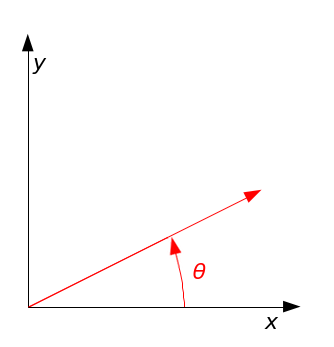
\includegraphics[scale= 0.5]{./figures/rotation}
 	\caption{The rotation in 2-D space, carried put by the rotation operator.}
 	\label{fig:rotation}
 \end{figure}
 \subsection{The differential operator}
 There are operators also acting on function space, they have the same properties as the operators discussed above, but with slight modifications. For example, the operators acting on function space cannot have an \textit{explicit} matrix representation. \\
 The most famous operators which act on function space are the differential operators; denoted by $ \hat{L}$. There are a variety of differential operators. They play an important r\^{o}le in the theory of differential equations. In fact, most of the problems in quantum mechanics are related to the analysis of the differential operators related to dynamical observables; as we shall see.\\
 Take the function $ f(x) = e^{ \lambda x}$. It is the eigenfunction of the differential operator $ \dfrac{d}{dx}$, with an eigenvalue $ \lambda$. Hence, we conclude that $e^{ \lambda x}$, is a solution to the differential equation:
 \begin{equation}
 \dfrac{d}{dx} ( f(x) = \lambda f(x)
 \end{equation}
 The operator $\dfrac{d^2}{dx^2}$ has two eigenfunctions $ e^{+ \lambda x}$ and $ e^{-\lambda x}$ they resemble solutions for the differential equation :
 \begin{equation}
 \dfrac{d^2}{dx^2} ( f(x) = \lambda f(x)
 \end{equation}
 And by the superposition principle, a general solution would be:
 \begin{equation}
 f(x) = A e^{+ \lambda x} + B  e^{-\lambda x}
 \end{equation}
 \section{ Commutators}
 Just like ordinary matrix multiplication, the product between operators is generally non-commutative. In fact, this particular property of operator multiplication is behind the unfamiliar phenomena observed in quantum mechanics, thus generally we have :
 \begin{equation}
 \hat{A} \hat{B} \neq \hat{B} \hat{A}
 \end{equation} 
 We define the \textbf{commutator} between two operators as:
 \begin{equation}
 [\hat{A}, \hat{B}] \equiv  \hat{A} \hat{B} - \hat{B} \hat{A}
 \end{equation}
 The commutator satisfies the following properties:\\
 \begin{tabular}{ll}
 	$ [\alpha A+ \beta B, C]= \alpha [ A,C]+\beta[B,C]$& linearity in both slots.\\
 	$[A,[B,C]] + [B,[C,A]] + [C,[A,B]] = 0$ & Jacobi Identity \\
 	$[AB,C] = [A,C]B + A[B,C]$& Product rule 
 \end{tabular}
 For the last property, it is a rule of thumb to think of the commutator as a kind of derivative $\mathcal{D}_C = [\cdot,C]$:
 \[
 \mathcal{D}_C \left( AB\right)  = \mathcal{D}_C (A)B +A \mathcal{D}_C (B)
 \]
 \section{Function of operator}
 Just like scalars, one can a function of an operator: $ f( \hat{A}) $ This is justified because, one can expand the function $ f( \hat{A}) $ as a series:
 \begin{equation}
 f( \hat{A}) \approx f_0I + f_1 \hat{A} + \frac{f_2}{2!} \hat{A}\hat{A} + \dots 
 \end{equation}
 Since operator product is defined, the function itself is well-defined as well\\
 Commutator of a function is given by :
 \begin{equation}
 [f(\hat{B}), \hat{A}] = \left( \dfrac{d f(\hat{B})}{d \hat{B}}\right)  [ \hat{B},\hat{A}]
 \end{equation}
 Provided that \[
 [ [ \hat{B},\hat{A}], \hat{A}] =0
 \]
 Another important formula to learn is the Hadamard Lemma:
 \begin{equation}
 e^{\hat{A}}\hat{B}e^{-\hat{A}}=\hat{B}+[\hat{A},\hat{B}]+\frac{1}{2!}[\hat{A},[\hat{A},\hat{B}]]+\dots
 \end{equation}
 \section{Commuting operators}
 For two commuting operators,
 \begin{equation}
 [\hat{A}, \hat{B}] =0
 \end{equation}
 one can find a common set of eigenbasis :
 \begin{align}
 \hat{A} | i\rangle &= a_i | i\rangle \\
 \hat{B} | i\rangle &= b_i | i\rangle 
 \end{align}
 The eigenkets form a mutual eigenbasis for the states $ \hat{A} | \psi\rangle$ and $ \hat{B} | \psi\rangle$. Hence one can simultaneously diagonalise both operators. 
 \section{Problems}
 \begin{enumerate}
 	\item Find the eigenvalues of the operator :
 	
 	\[ \hat{A} =
 	\begin{pmatrix}
 	1& i&0\\
 	-i&2&-i\\
 	0&i&1
 	\end{pmatrix}
 	\]
 	Can we diagonalise it ?.
 	\item Is the operator $ d/dx$ acting on the $ L^2$ Hilbert space hermitian ? How about $ -i d/dx $ ?
 	\item Show that for a Hermitian operator $ \hat{T}$ the operator $ \hat{U}\equiv e ^ {i \hat{T}}$ is unitary.
 	\item Is the function $ \cos{kx}$ an eigenfunction for the operator $ d/dx$ ?  What about the operator $ d^2/dx^ 2$ ?
 	\item Show that for an operator $ \hat{A}$ commuting with the \textbf{Hamiltonian operator} $ \hat{H}$ we can write its time evolution as:
 	\[
 	e^{i\hat{H} t} \hat{A} e^{-i\hat{H} t}
 	\]
 	\textit{Hint: use Hadmard lemma}
 	This is known as \textbf{Heisenberg equation}
 	\item We define the expected value - average value- of an operator with respect to a state vector $ | \psi \rangle$ as:
 	\[
 	\langle \hat{A}\rangle \equiv\langle\psi|\hat{A} | \psi \rangle
 	\]
 	Show that if  $ | \psi \rangle$ is expanded in terms of the eigenbasis of $\hat{A}$, then the expected value is the sum of the eigenvalues of the operator $ a_n$, i.e. 
 	\[
 	\langle \hat{A}\rangle = \sum_n c_n a_n
 	\]
 	for some constants $c_n$.
 	\item Recall that we defined the identity operator as the outer product of the basis :
 	\[
 	I = \sum_i |i\rangle\langle i|
 	\]
 	Using this definition, show that this operator sends the ket $ | \psi\rangle$ to itself ( does not change the ket), then show this for the Bra vector $\langle \psi|$.
 	\item Discuss why if $ [ \hat{A}, \hat{B}] | \psi\rangle \neq 0 $ one cannot find a mutual eigenbasis to expand $| \psi\rangle$ with ?
 \end{enumerate}